\subsubsection{\stid{1.17} Open~MPI for Exascale (OMPI-X)}\label{subsubsect:openmpi}

%% {\itshape

%% 	\begin{enumerate}
%% 	\item Rename this file to your project WBS-projectname.tex, for example 2.3.3.01-XSDK4ECP.tex.
%% 	\item Complete this template for your project.  Limit your text to two pages, not counting citations.
%% 	\item Please avoid changing the content of main.tex.
%% 	\item Put any references in a .bib file with the same root name, for example 2.3.3.01-XSDK4ECP.bib.
%% 	\item Remember to include any image files you reference in your text.
%%     \item The files 2.3.3.01-XSDK4ECP.tex, 2.3.3.01-XSDK4ECP.bib and xSDK-diagram.jpeg are included as examples for your reference.  You can remove them from what you upload.
%% 	\end{enumerate}
%% }

\paragraph{Overview}
%% \textit{Provide an overview of your project.  You might find that the introductory text from your Fall 2017 Project Summary \url{https://confluence.exascaleproject.org/display/1ST/Fall+2017+ECP+ST+Project+Summaries} useful as a starting draft.}

The OMPI-X project ensures that the Message Passing Interface (MPI)
standard, and its specific implementation in Open~MPI meet the needs
of the ECP community in terms of performance, scalability, and
capabilities or features. MPI is the predominant interface for
inter-process communication in high-end computing.  Nearly all of the
ECP application (AD) projects (93\%~\cite{Bernholdt:2018:SMU-tr})
and the majority of ST projects
(57\%~\cite{Bernholdt:2018:SMU-tr}) rely on it.
With the impending exascale era, the
pace of change and growing diversity of HPC architectures pose new
challenges that the MPI standard must address.  The OMPI-X project is
active in the MPI Forum standards organization, and works within it to
raise and resolve key issues facing ECP applications and libraries.

Open~MPI is an open source, community-based implementation of the MPI
standard that is used by a number of prominent
HPC vendors as the basis for their commercial MPI offerings.   The
OMPI-X team is comprised of active members of the Open~MPI community,
with an extensive history of contributions to this community.
The OMPI-X project focuses on prototyping
and demonstrating exascale-relevant proposals under consideration by
the MPI Forum, as well as improving the fundamental performance and
scalability of Open~MPI, particularly for exascale-relevant platforms
and job sizes.
MPI users will be able to take advantage of these
enhancements simply by linking against recent builds of the Open~MPI
library.

In addition to MPI and Open~MPI, the project also includes two other products,
which are less visible to the end user, but no less important.
PMIx (Process Management Interface for Exascale) provides facilities for
scalable application launch, process wire-up, resilience, and coordination between runtimes.
It originated as a spin-off from the Open~MPI community, but is now developing a
community of its own as adoption grows.  Starting in FY20,
Qthreads (formerly WBS 2.3.1.15) is also part of the OMPI-X project.  Qthreads is a
user-level lightweight asynchronous thread library particularly focused on improving support for
multithreading in the context of network communications.  Both PMIx and Qthreads help the
OMPI-X project address key issues of performance and capability for exascale applications.


\paragraph{Key  Challenges}
%% \textit{Describe what is hard to do, why it is challenging.}
A number of aspects of ``exascale'' levels
of computing pose serious challenges to the ``tried and true'' message
passing model presented by MPI and its implementations, including Open~MPI.
%
Keeping pace with changes in HPC architecture is a major challenge.
Examples include massive node-level concurrency, driving the
growth of ``MPI+X'' programming approaches,
and the complex memory architectures, which make the placement of data
within memory more important. In the near-term, with GPUs dominating the exascale
environment, how code running on the GPUs interacts with MPI and inter-process
communications must also be addressed.  This will require both changes to the standard
and changes and improvements within implementations.
%
Performance and scalability become both more important and more
challenging as node counts increase
and memory per MPI rank trends downward.
%
Finally, as we identify solutions to these challenges that must be
``implemented'' within the MPI \emph{standard} rather than particular MPI libraries,
we must work within the much larger and broader MPI
community that may not always be attuned to the needs of computing at the largest scales.

\paragraph{Solution Strategy}
%% \textit{Describe your basic strategy for addressing the challenges.}
The OMPI-X project is working across a number of fronts to address
these challenges.

\emph{Runtime Interoperability for MPI+X and Beyond} MPI is
increasingly being used concurrently with other runtime environments.
This includes both ``MPI+X'' approaches, where X
is most often a threading model, such as OpenMP, as
well as the use of multiple inter-process runtimes within a single
application.  Concerns include awareness of other runtimes,
cooperative resource management capabilities, and ensuring that all
concurrently active runtimes make progress.  We are developing APIs and
demonstrating capabilities for interoperability in both MPI+X and
multiple inter-process runtime situations.

\emph{Extending the MPI Standard to Better Support Exascale
Architectures} The MPI community is standardizing a
number of ideas that
are particularly important to supporting
the architectural and system size characteristics anticipated for
exascale.  ``Partitioned communications'' (previously called ``Finepoints'')
deal with the growing use of threading for node-level concurrency, in
combination with MPI.  ``Sessions'' increases the flexibility of MPI
semantics in a number of areas, which in turn can open opportunities
for enhanced scalability, as well as easier support for
multi-component applications such as coupled multi-physics
simulations. Error management and recovery capabilities are key to
ensuring that applications can detect and respond effectively when errors,
inevitably, occur during execution.  We are helping to drive incorporation
of these and other ideas into the MPI standard by developing prototypes and
working with ECP teams and the broader community to demonstrate their
feasibility and value.

\emph{Open~MPI Scalability and Performance} As we push the scale of
both hardware and applications, we stress MPI implementations and
expose areas that need to be improved.
OMPI-X is targeting key components within Open~MPI, such as threading capabilities,
memory usage, remote memory access (RMA), tag matching, and other areas,
for improvements in both scalability and performance.

\emph{Supporting More Dynamic Execution Environments} We are
developing and implementing strategies to help MPI applications
better deal with topological process layout preferences
and contention in the network.

\emph{Resilience in MPI and Open~MPI} Concerns about system and
application resilience increase as either scales in size.  Our goal in
this area is to ensure that MPI, Open~MPI, and PMIx provide not only
support for simplified
recovery for the widely used checkpoint/restart fault tolerance strategy, but also the building
blocks to support more general error management and recovery by applications (the evolution of the User-Level
Fault Mitigation concept). We work within the MPI Forum, implement,
and train users on resilience strategies.

\emph{MPI Tools Interfaces}  Several interfaces within the
MPI standard are primarily used to support performance and
correctness tools.
The MPI Forum is in the process
of making significant revisions and extensions to these interfaces.
We will track the discussions in the Forum and provide prototype
implementations within Open~MPI to facilitate evaluation and provide
feedback.
We will work with the
ECP community, including tool developers, to make additional data
available through the MPI\_T interface.

\emph{Quality Assurance for Open~MPI}  We are enhancing the
Open~MPI testing infrastructure, adding tests to reflect ECP
requirements, and instantiating routine testing on systems of
importance to ECP, both for correctness and performance.

\begin{wrapfigure}{r}{0.40\textwidth}
    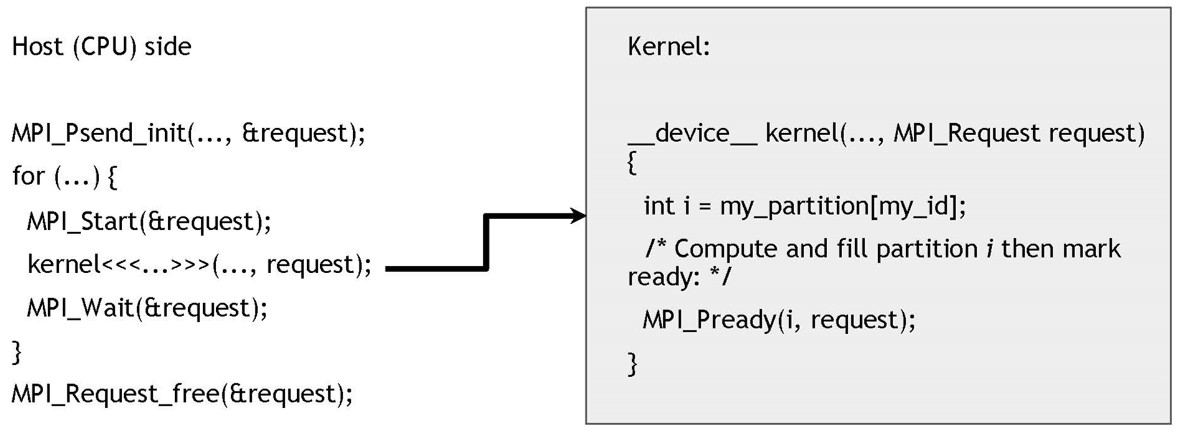
\includegraphics[width=0.40\textwidth]{projects/2.3.1-PMR/2.3.1.17-OMPI-X/partitioned-comms-code.jpg}
    \caption{Schematic code illustrating use of partitioned communications from a GPU kernel.  
    Host code (left) sets up communication, GPU kernel (right) triggers send (MPI\_Pready).}
    \label{fig:partitioned-communications}
\end{wrapfigure}

\paragraph{Recent Progress}
%% \textit{Describe what you have done recently.  It would be good to
%% have some kind of figure or diagram in this section.}
The MPI Forum finalized and released version 4.0 of the standard in June 2021.  The OMPI-X team helped drive
the incorporation a number of new features and capabilities considered important for exascale applications.
These include sessions and a number of error management and recovery features
based on the long-standing User-Level Fault Mitigation (ULFM) concept.  Partitioned communications (Fig.~\ref{fig:partitioned-communications})
is another major addition to the standard which is designed to benefit massively-threaded environments, such as GPU accelerators, by supporting
incremental completion of the communication as portions of the buffer become ready.
These capabilities have at least prototype-level implementations available in the Open~MPI library, allowing interested project teams to start
exploring the new capabilities.  

As the MPI Forum continues its work beyond 4.0, the OMPI-X team continues 
its strategic involvement on topics that did not make the 4.0 release of the standard or further enhancements to 4.0 features
to improve support for high-end systems and the ECP community,  particularly in the context of resilience. The ULFM
proposal has been updated to reflect those features that have been incorporated into 4.0, as well as the discussions
within the Forum.  For the complementary Reinit simplified checkpoint/restart proposal (Figure~\ref{fig:reinit}), we have carried out a formal verification on the recovery algorithm. 
This ensures that the protocol, which we plan to propose for a future version of MPI, correctly handles the recovery phase 
of a failure response, including correct propagation of notifications, absence of deadlocks, and proper termination.
During the past year, the Reinit recovery protocol has been formally verified
and a prototype implementation has been developed in Open~MPI.  Performance evaluation
of the approach show it offering superior performance to traditional checkpoint/restart
for the HPCG benchmark against different types of failures (Fig.~\ref{fig:reinit}).

\begin{figure}
    \centering
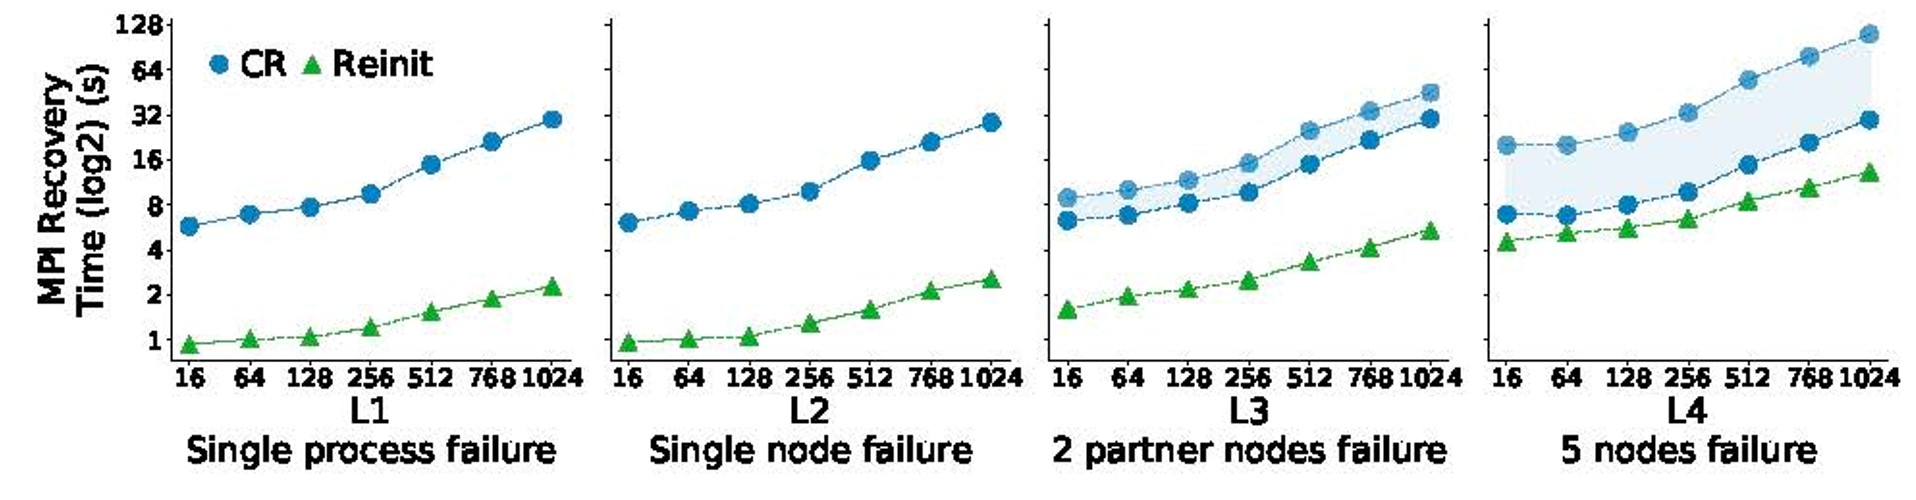
\includegraphics[width=0.80\textwidth]{projects/2.3.1-PMR/2.3.1.17-OMPI-X/reinit-performance.jpg}
\caption{Comparison of recovery times for traditional checkpoint/restart (blue) and Reinit (green) for the HPCG benchmark.  
Each graph represents different types/severities of failures.}
\label{fig:reinit}
\end{figure}

As part of the larger Open~MPI community, we are working towards a major-version
release (v5.0.0), planned for late CY2021.  This release will include many contributions
of the OMPI-X team, including the beginnings of our work towards full support for
MPI 4.0, user-level fault mitigation and FP16 support (both of which we will be advocating
for future MPI standards), and performance enhancements such as SIMD support for MPI reductions,
and improvements to collective and atomic operations.

\begin{wrapfigure}{r}{0.40\textwidth}
    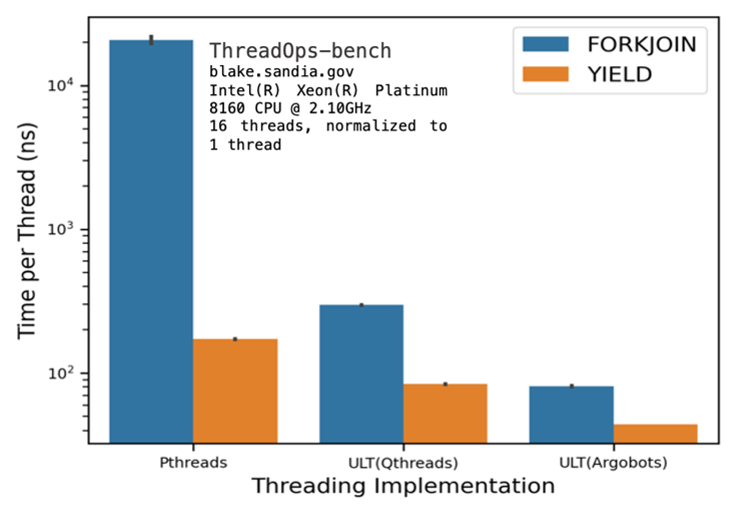
\includegraphics[width=0.40\textwidth]{projects/2.3.1-PMR/2.3.1.17-OMPI-X/ult-performance.png}
    \caption{Illustration of relative costs of PThreads vs ULT threads (Qthreads, Argobots) using ThreadOps benchmark for fork-join and yield operations.}
    \label{fig:ult-performance}
\end{wrapfigure}

To support highly-threaded ``MPI+X'' use cases primarily on the CPU side, the OMPI-X project has teamed with the MPICH and Argobots ECP teams (WBS 2.3.1.07 and 2.3.2.11)
to define interfaces in both MPICH and Open~MPI to support the use of lightweight user-level threading (ULT) libraries such as Qthreads or BOLT
as an alternative to Pthreads.  The new ULT support, now integrated into both libraries, offer significantly improved performance compared to 
the traditional Pthreads implementation (Fig.~\ref{fig:ult-performance}).

Another key product that the OMPI-X project supports is the Process Management Interface for Exascale (PMIx).  PMIx includes both a community standard
and a reference implementation, OpenMPIx.  Open~MPI relies on the PMIx standard and the PRRTE reference runtime for process startup, wireup, and runtime coordination.
It is also used and implemented by a variety of other libraries and projects, including LLNL's Flux resource manager (WBS 2.3.6.02), which is in turn part of the ExaWorks toolkit (WBS 2.3.5.10).
During the past year, version 4.0 of the PMIx standard was released, as well as version 4.1.0 of OpenPMIx and version 2.0.0 of PRRTE.

In addition to these activities, we continue to support quality assurance of the Open~MPI code base through more and better testing.  The Open~MPI testing infrastructure, 
MTT, continues to be improved for flexibility and capability.  One of this year's noteworthy efforts was the addition of the bueno application test harness to the testing 
system.  The facilitates incorporating third-party test cases (i.e. based on user applications) into the routine testing process without having to commit them to the
Open~MPI testing repository.  We are also working to establish more frequent testing regimes on key DOE hardware platforms.

\paragraph{Next Steps}
%% \textit{Describe what you are working on next.}
The delivery of the first HPE Slingshot-11 (SS-11) network, as part of the Frontier system, at the beginning of FY22 finally affords us
the opportunity to start our work to ensure that Open~MPI provides good support for SS-11, which we expect to be the focus of significant
effort this year.  SS-11 will be used on both Frontier and Aurora, so much of the work will support both systems, though there will be differences 
in on-node (particularly GPU-to-GPU) transfers due to the different GPU accelerators.  The different workload management solutions on the two platforms
will also need to be supported.  Additionally, we will be in a much better position to work with application teams who can benefit from the new capabilities 
embodied in MPI 4.0, but who have been reluctant to adopt them until they were officially part of the standard.  
We will likewise continue to identify and improve performance and scalability bottlenecks and drive forward on
the core themes outlined in our Solution Strategy.

\paragraph{Early Access System Experience}
Most of the early access systems have utilized InfiniBand interconnects, which are well-supported 
by Open MPI (the HPE Slingshot-10 interconnect is also InfiniBand).  The Frontier test and development
system Crusher was the first system available with the new Slingshot-11 network.  A subset of the
OMPI-X team obtained access to Crusher in December, and have been working to port Open MPI to
the SS-11 interconnect.  The basic approaches available leverage either Open Fabric providers or
the UCX communication infrastructure, or some combination.
So far, we've confirmed basic point-to-point functionality using the HPE-provided
CXI Open Fabric provider, and partial intra-node shared memory functionality through the 
UCX communications framework.
We plan to continue exploring all three paths until we arrive at a solution that provides full functionality
with the expected performance.

The Qthreads user-level lightweight threading package is not dependent on the network, nor on the GPUs
so it is easier to port.  It has been confirmed to work on Spock (the Frontier early access system).
Challenges getting the Qthreads team access to ANL early access systems have delayed demonstration
of the functionality there, but we do not anticipate any problems.  The team just recently obtained
access to Arcticus and plans to test Qthreads there shortly.
